\documentclass[border=10pt]{standalone}
\usepackage{pgfplots}
\usepackage{siunitx}
\pgfplotsset{width=7cm,compat=1.8}
\usepgfplotslibrary{polar}
\pgfplotsset{mypolarplot/.style={%
  clip=false, % needed for double line (last \addplot command)
  domain=0:360, % plot full cycle
  samples=300, % number of samples; can be locally adjusted
  grid=both, % display major and minor grids
  major grid style={black}, 
  minor x tick num=3, % 3 minor x ticks between majors
  minor y tick num=1, % 1 minor y tick between majors
  xtick={0,90,...,359},
  xticklabels={%
    $\theta = \ang{0}$,
    $\theta = \ang{90}$,
    $\theta = \ang{180}$,
    $\theta = \ang{270}$
  },
  yticklabel style={anchor=east}, % move label position
}}
\begin{document}
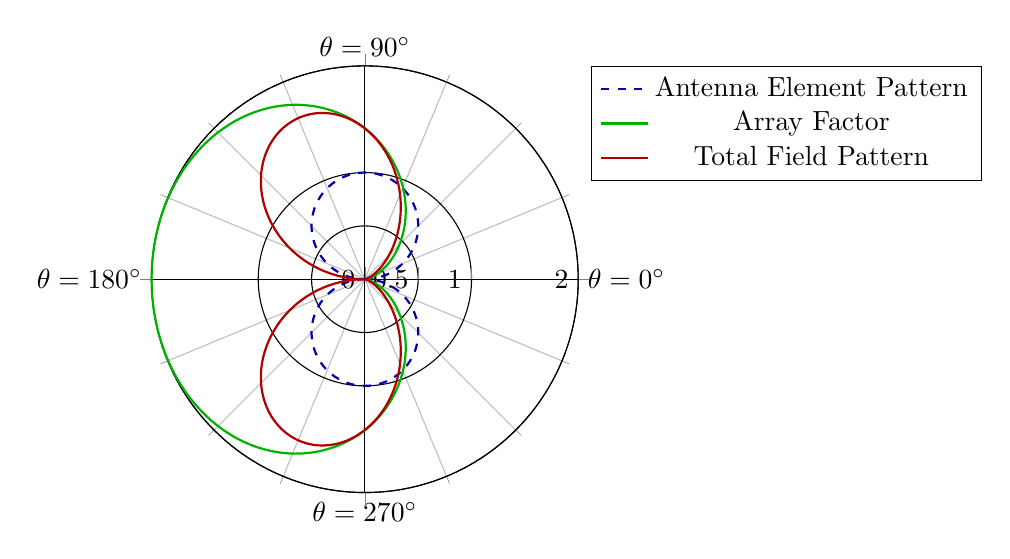
\begin{tikzpicture}

    \pgfmathsetmacro{\alpha}{90}
      \pgfmathsetmacro{\d}{1/4}
    \begin{polaraxis}[%
        ymax=2,
        ytick={0,.5,1,2},
        mypolarplot,legend pos=outer north east
      ]

      \addplot[mark=none,blue!70!black,dashed,thick] 
      {abs(sin(\x))};

      \addplot[mark=none,thick,green!70!black] 
      {(2*cos(1/2*(2*180*\d*cos(\x)+\alpha)))}; 


        \addplot[mark=none,thick,red!70!black] 
        {abs(sin(\x))*(2*cos(1/2*(2*180*\d*cos(\x)+\alpha)))}; 
    \addlegendentry{Antenna Element Pattern}
   \addlegendentry{Array Factor}
   \addlegendentry{Total Field Pattern}
; % there is likely a better way to do this
      \end{polaraxis}
\end{tikzpicture}
\end{document}